\section{概念}

\subsection{概念(広辞苑)}
事物の本質をとらえる思考の形成。事物の本質的な特徴とそれらの連関が概念の内容(内包)。概念は同一本質をもつ一定範囲の事物(外延)に適用されるから一般性をもつ。例えば、人という概念の内包は人の人としての特徴であり、外延はあらゆる人々である。しかし、個体(例えばナポレオン)をとらえる概念(個体概念・単独概念)もある。概念は言語に表現され、その意味として存在する。概念の成立については哲学に共通する内容をとりだし(抽象)、個々の事物にのみ属する偶然的な性質をすてる(捨象)ことによるとするのが通常の見解で、これに対立するものが経験から独立した概念(先天的概念)を認めた立場。\\

\subsection{概念の現状}
概念は、現在様々な使われ方をしている。一般に人間が上記の日本語の「概念」として用いられている場合と、次節で示される「概念そのものの概念」である。\\

\subsubsection{概念の概念}
概念の概念。それは通常の概念の概念ではなく、概念そのもの概念の本質に迫る概念である。現在、世界中の物理学者がこの問題について研究しており、様々な研究成果が報告されている。知らんけど。

\subsubsection{という概念}
近年ではあまり観測されない現象ではあるが、主に2015年、神戸大学の粒子物理研究室においてぐっさんにより観測された。何かしらの事象に対する呼応反応として「◯◯という概念。{\sf (´\_ゝ`)}笑」とか言ったりしてたっていう。

\subsubsection{概念方程式}
後述。知らんけど\sf(´\_ゝ`)

\newpage
\subsection{概念方程式}
\subsubsection{概念方程式(創世記)}
「概念の規格化」という概念が存在した。

\subsubsection{概念方程式(爆発)}
「概念の概念」という概念が爆誕した。

\subsubsection{概念方程式(整備)}
重症患者により概念についての整備がされ、以下で示される概念が明記された。

\begin{eqnarray}
{概念}^{概念}=?
\end{eqnarray}

\subsubsection{概念方程式(完成)}
重症患者により概念についての整備がなされた結果、以下で示される概念方程式が完成した。


\begin{eqnarray}
{概念1}^{概念2}={概念1}\times{概念2}
\end{eqnarray}

世界中の様々な重症患者達がこの概念方程式を解こうとしたが、未だかつて解かれておらず、概念の概念はどういう概念なのかとかそういう概念が概念概念していたという概念\sf{ (´\_ゝ`)}

\newpage
\subsection{概念方程式の解}
概念方程式を解いていく上で、概念における様々な定義の概念と公理の概念が必要であった。よってそれを以下に示す。

\subsubsection{定義}

\begin{eqnarray}
{概念1}\equiv G_{1}
\end{eqnarray}\footnote{概念の添字である数字は佐藤パラメータと呼ぶ}

\begin{eqnarray}
{概念2}\equiv G_{2}
\end{eqnarray}

\begin{eqnarray}
G_{1}^{G_{2}}=G_{1}G_{2}
\end{eqnarray}

\subsubsection{公理}
\begin{itembox}[c]{鈴木州のたこ鍋徹夜}
なんかもう一つ方程式ないとあかんやんとか言ってたら州がこんなん言いだした。
\begin{eqnarray}
\mathcal{L}(G_{i+1})=\frac{1}{G_{i}}
\end{eqnarray}
\end{itembox}

\begin{itembox}[c]{又吉先生のn}
後々なんかn=0であって欲しい場面が出てくるが、その理由を又吉先生に聞いたらこんなこと言ってた。
\begin{eqnarray}
n = 得ぬ = 0
\end{eqnarray}
\end{itembox}

\newpage
\subsection{解法}
概念方程式を徐々に解いていく。

\begin{eqnarray}
G_{1}^{G_{2}}&=&G_{1}G_{2}\\
\raisebox{.2ex}{.}\raisebox{1.2ex}{.}\raisebox{.2ex}{.}  G_{2}ln{G_{1}}&=&ln{G_{1}}+ln{G_{2}}\\
\end{eqnarray}

normalized to $G_{1}$

\begin{eqnarray}
ln{G_{1}}&=&\frac{1}{G_{2}}ln{G_{1}}+\frac{1}{G_{2}}ln{G_{2}}\\
\raisebox{.2ex}{.}\raisebox{1.2ex}{.}\raisebox{.2ex}{.} ln{G_{1}}(1-\frac{1}{G_{2}})&=&\frac{1}{G_{2}}ln{G_{2}}\\
\raisebox{.2ex}{.}\raisebox{1.2ex}{.}\raisebox{.2ex}{.} ln{G_{1}}\times (1-\frac{G_{2}-1}{G_{2}})&=&\frac{1}{G_{2}}ln{G_{2}}\\
\raisebox{.2ex}{.}\raisebox{1.2ex}{.}\raisebox{.2ex}{.} ln{G_{1}}&=&\frac{1}{G_{2}-1}ln{G_{2}}\\
\raisebox{.2ex}{.}\raisebox{1.2ex}{.}\raisebox{.2ex}{.} ln{G_{1}}&=&ln{G_{2}^{\frac{1}{G_{2}-1}}}\\
\raisebox{.2ex}{.}\raisebox{1.2ex}{.}\raisebox{.2ex}{.} G_{1}&=&G_{2}^{\frac{1}{G_{2}-1}}
 \end{eqnarray}

generalizing,

\begin{eqnarray}
\raisebox{.2ex}{.}\raisebox{1.2ex}{.}\raisebox{.2ex}{.} G_{i}&=&G_{i+1}^{\frac{1}{G_{i+1}-1}}
 \label{i1}
 \end{eqnarray}

so,it could be  derived the relation between $G_{i}$ and $G_{i+1}$.\\
\\
ところで、式\ref{i1}から一般概念$G_{n}$を求めようとした場合、簡単にはいかない。ここで、以下で示されるシステム「Wolfram Alpha」を導入する。\\

\newpage
\subsubsection{Wolfram Alpha}
Wolfram Alpha(WolframAlphaともWolfram|Alphaとも表記される)はウルフラム・リサーチが開発した質問応答システム。事実についての質問に対して、構造化されたデータを使って計算し、直接答えを返すオンラインサービスである。他の検索エンジンのように、答えを含んでいる可能性のあるドキュメントやウェブページのリストを返すわけではない[3]。このサービスは2009年3月に英国人科学者スティーブン・ウルフラムが発表し、同年5月15日に公開された[1]。
\begin{itemize}

\item 概要\\
ユーザはテキストフィールドに質問や計算リクエストを入力して送信する。Wolfram Alphaは知識ベースの精選された構造化データから答えと関連する視覚的情報を計算する。ゆえにWolfram Alphaは、多数の答えのインデックスを作成し、質問をいずれか1つに合致させようとするセマンティック検索エンジンとは異なる。\\
 Wolfram Alphaはコンピュータ代数、記号および数値計算、可視化、統計などの機能を網羅するウルフラムのフラッグシップ製品Mathematicaの上に構築されている。答えは通常読みやすい形の解で示される。\\
例:「lim(x->0) x/sin x」は正しい結果1に加え、ロピタルの定理を使った微分、プロット、そして級数展開を返す。\\
 Wolfram Alphaは自然言語を使った、事実についての質問にも答えることができる。例えば、「Where was Mary Robinson born?」(メアリー・ロビンソンが生まれた場所は?)や、より複雑な「How old was Queen Elizabeth II in 1974?」(1974年時点でエリザベス2世は何歳?)などである。 (ロビンソンについての答えには「Ballina, Mayo, Ireland」(アイルランドのメイヨー州バリナ)、バリナについてのさまざまな情報、ロビンソンについてのオンラインの略歴へのリンクが含まれる。エリザベス女王についての答えは「Result for start of 1974: 47 years」(1974年の始まりの時点で47歳)と略歴へのリンクである。)
複数のソースのデータを使って計算を行うこともできる。
例:「What is the fifty-second smallest country by GDP per capita?」(国民1人あたりの国内総生産が52番目に小さい国は?)と入力すると、ニカラグアで年1160ドルであると返される。\\
Wolfram|Alphaは少量の中核となる情報から推定を行う。 この点において、Wolfram Alphaは1980年代に始まった一般常識推論エンジンの開発に焦点をあてたプロジェクトCycとの多くの類似点がある。\\
データベースには、現在、現在および過去の天候情報など、何百ものデータセットが含まれている。このデータセットは2年以上かけて蓄積されており、今後も増える予定である。データセットの増加に従って答えられる問題の範囲も広がっていく予定である[4] 。

\item ライセンスパートナー\\
Wolfram AlphaはMicrosoft BingおよびDuckDuckGo検索エンジンの検索機能を提供している[5][6]。\\
Wolfram AlphaはAppleのSiri、DexetraのAndroid Irisから、事実に基づく質問に対する回答を受ける。\\
\item テクノロジー\\
Wolfram|AlphaはwebMathematicaとgridMathematicaを使って1500万行のMathematicaコードで書かれており[7]、1万個のCPU(この個数は起動に向けて拡張された)上で実行されている[8][9]。

\item 起動\\
 起動準備は中部標準時で2009年5月15日午後7時(16 May 2009 0:00 UTC)に始まり、Justin.tvでライブ放送された。高負荷問題を予想しながらも、その数時間後から公式起動する予定であった。このサービスは2009年5月18日に公式に起動した[10]。\\
Wolfram Alphaについては肯定的な評価がなされている[11][12]。 Wolfram Alphaの支持者の中には、将来性を評価する人や、現在の有用性よりWolfram Alphaが結果を導くその工程が重要なのだと指摘する人もいる[11]。
\item Wolfram Alpha Pro\\
2012年2月8日,Wolfram|Alpha Proが発表された[13]。これは月々の利用料によってユーザに追加機能を提供するものである。主な機能には、表形式、画像、音声、XML、何十もの特化した科学・医用・数学形式など、一般によく使われる多くのファイル形式をアップロードして自動的に解析することができるというものがある。その他には、拡張キーボード、CDFを使ったインタラクティブ機能、データのダウンロード、グラフィックスや表を含む結果をカスタマイズして保存できる機能などがある[14]。
Wolfram Alpha Proの新しいプレミアム機能の導入に伴い、無料ページにいくつかの変更点が加わった。
無料サイトの広告が増えた。
テキストとPDFによるエキスポート機能を利用するためには、無料アカウントが必要になった。
時間のかかる計算のための計算時間延長のリクエストは以前は無料[15]であったが、購読者のみが対象となった[16]。
\end{itemize}


\newpage
以上のWolfram Alphaをいそべっちがぐぐってなんか計算してくれたのを参考$\sf{ (´\_ゝ`)}$にし、計算を続けた。その結果、図\ref{wolfram}のような結果となった。\\
\begin{figure}[H]
\centering
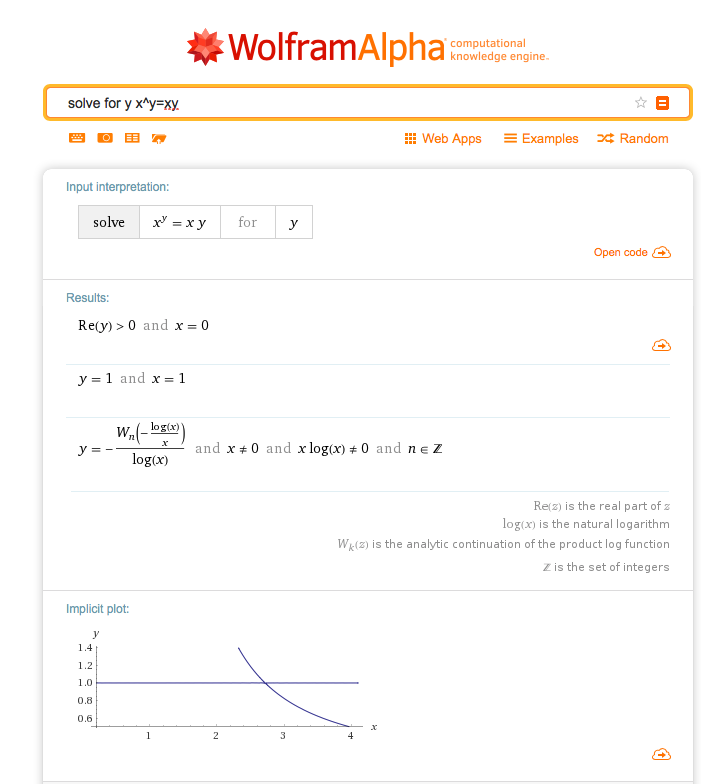
\includegraphics[clip,scale=0.35]{wolfram.png}
    \caption{Wolfram Alpha}
    \label{wolfram}
\end{figure}

これより、式\ref{i1}から一般概念$G_n$を求めると式\ref{i2}で表される。

\begin{eqnarray}
G_{i+1}=-\frac{W_{n}\left( -\frac{logG_{i}}{G_{i}}\right)}{logG_{i}} \ \ \ \ 
\label{i2}
 \end{eqnarray}

ここで$W_n$はランベルトのW関数である。

\newpage
\subsubsection{ランベルトのW関数}
数学におけるランベルトW函数(ランベルトWかんすう、英: Lambert W function)あるいはオメガ函数 ($\omega$function), 対数積(product logarithm; 乗積対数)は、函数 f(z) = zez の逆関係の分枝として得られる函数 W の総称である。ここに ez は指数函数で z は任意の複素数とする。すなわち W は z =$f_{−1}(zez)$=W(zez) を満たす。
上記の方程式で z' = zez と置きかえれば、任意の複素数 z' に対する W 函数(一般には W 関係)の定義方程式
\begin{eqnarray}
z'=W(z')e^{W(z')} 
\label{i3}
 \end{eqnarray}

を得る。
函数fは単射ではないから、関係Wは(0を除いて)多価である。仮に実数値のWに注意を制限するとすれば、複素変数zは実変数xに取り換えられ、関係の定義域は区間x$\leq$−1/eに限られ、また開区間 (−1/e,0) 上で二価の函数になる。さらに制約条件として W$\leq$−1 を追加すれば一価函数$W_{0}(x)$が定義されて、$W_{0}(0) = 0$および$W_{0}(−1/e) = −1$を得る。それと同時に、下側の枝は W$\leq$−1であって、$W_{−1}(x)$と書かれる。これは$W_{−1}(−1/e)=−1$から$W_{−1}(−0)=−\infty$まで単調減少する。
ランベルトW関係は初等函数では表すことができない。ランベルトWは組合せ論において有用で、例えば木の数え上げに用いられる。指数函数を含む様々な方程式(例えばプランク分布、ボーズ-アインシュタイン分布、フェルミ-ディラック分布などの最大値)を解くのに用いられ、また$y'(t) = ay(t − 1)$のような遅延微分方程式(英語版) の解としても生じる。生化学において、また特に酵素動力学において、ミカエリス-メンテン動力学の経時動力学解析に対する閉じた形の解はランベルトW函数によって記述される。知らんけど\sf (´\_ゝ`)笑

\newpage
\subsubsection{一般概念解}
以上を用いて一般概念解を求めていく。\\
まず、概念方程式より

\begin{eqnarray}
G_{i}^{G_{i+1}}&=&G_{i}G_{i+1}
 \end{eqnarray}

一方で、鈴木州のたこ鍋徹夜より、
\begin{eqnarray}
左辺&=&\mathcal{L}(G_{i+1})\nonumber\\
&=&\int^{\infty}_{0}G_{i+1}e^{-it}dt\nonumber\\
&=&G_{i+1}\int^{\infty}_{0}e^{-it}dt\nonumber\\
&=&G_{i+1} \frac{1}{-i} \left[ e^{-it} \right]^{\infty}_{0} \nonumber\\
&=&-iG_{i+1}\\
\raisebox{.2ex}{.}\raisebox{1.2ex}{.}\raisebox{.2ex}{.} \ -iG_{i+1}&=&\frac{1}{G_{i}}\nonumber\\
\raisebox{.2ex}{.}\raisebox{1.2ex}{.}\raisebox{.2ex}{.} \ G_{i}G_{i+1}&=&i
\label{i4}
\end{eqnarray}

となる。\\
また、又吉先生のnの概念を導入するとn=0になり、ランベルトのW関数に対して$W_{0}$の0を中心とするテイラー級数を逆に解いて近似すると

\begin{eqnarray}
W_{0}(x)&=&\sum^{\infty}_{n=0}\frac{(-n)^{n-1}}{n!}x^n\nonumber\\
&=&x-x^2+\frac{3}{2}x^3-\frac{8}{3}x^4+\frac{125}{24}x^5...\nonumber\\
&\sim&x
 \end{eqnarray}

となるので、式\ref{i2}について、
\begin{eqnarray}
G_{i+1}&=&-\frac{W_{0}\left( -\frac{logG_{i}}{G_{i}}\right)}{logG_{i}} \nonumber\\
&=&\frac{-1}{logG_{i}}\times -\frac{logG_{i}}{G_{i}}\nonumber\\
&=&\frac{1}{G_{i}} \nonumber\\
\raisebox{.2ex}{.}\raisebox{1.2ex}{.}\raisebox{.2ex}{.} \ G_{i}G_{i+1} &=& 1
\label{i5}
 \end{eqnarray}

と表される。\\
以上の式\ref{i4}、\ref{i5}より、
\begin{eqnarray}
\Large{i=1}
 \end{eqnarray}

となり、概念の概念から、「愛は一つ」ということが示された。またっっっっっっ\sf{ (´\_ゝ`)}笑

%%%%%%%%%%%%%%%%%%%%%%%%%%%%%%%%%%%%%%%%%%%%%%%%%%%%%%%%%
